\section{Metodology and Results}



\subsection*{3.1 Pump Integration}

    The pump integration in the automation algorithm bring us a new controllable variable, the Flowrate. Now we can control the spraying mode with the
    two main variables that afect the system. 
    It will bring more complexity for the system since now we are dealing with multivariable control.
    Fortunatelly those two variables are uncuppled (* be certain of that first *) which means that actuating in one of them will not interfere in the other one.
    Controlling also the flowrate gives to this project a new dimension in the system giving us freedom to explore the flowrate properties.

    The pump integration was developed using also python language. As I could not find a good library for this pump I developed an quick and easy interface for sending the pump
    commands to be integrated with the main automation routine. The communication with the pump was made using the serial interface and the commands list were found in the pump user manual.


\subsection*{3.2 First mapping Experiments}


    \begin{figure}[H]
        \center
        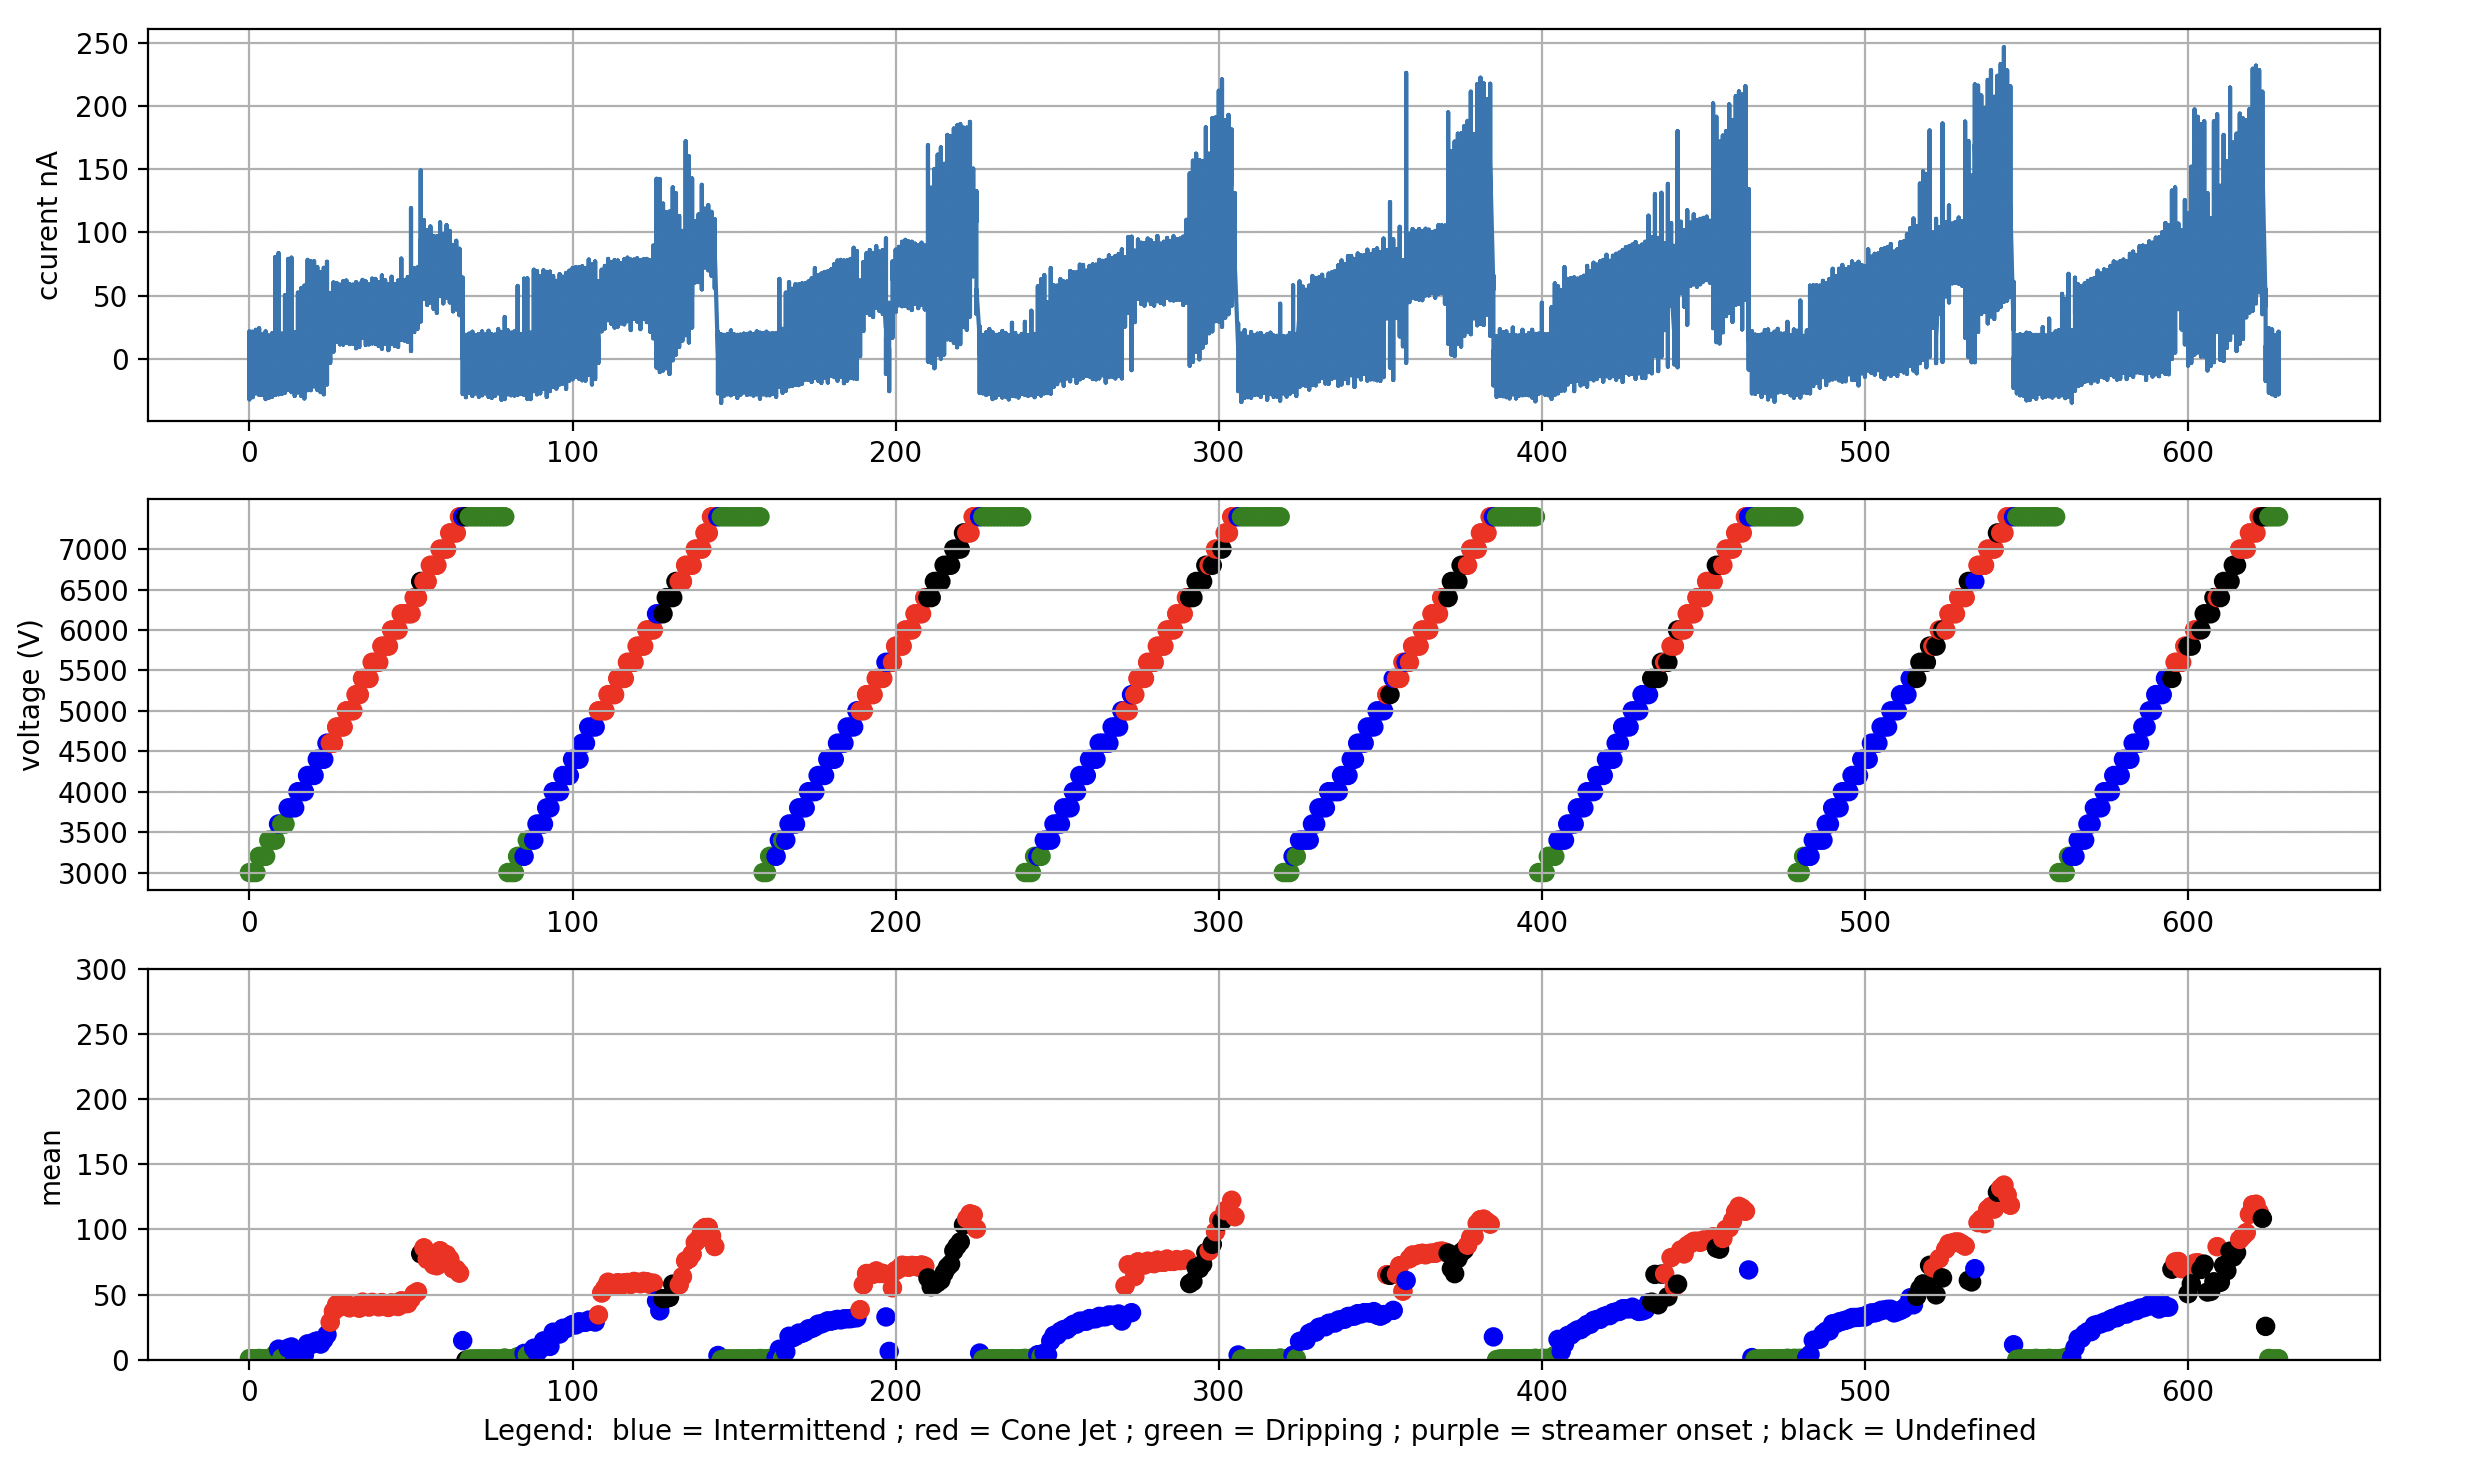
\includegraphics[width=15cm]{images/map2Data.png}
        \caption{Mapping Experiment data}
    \end{figure}

    \begin{figure}[H]
        \center
        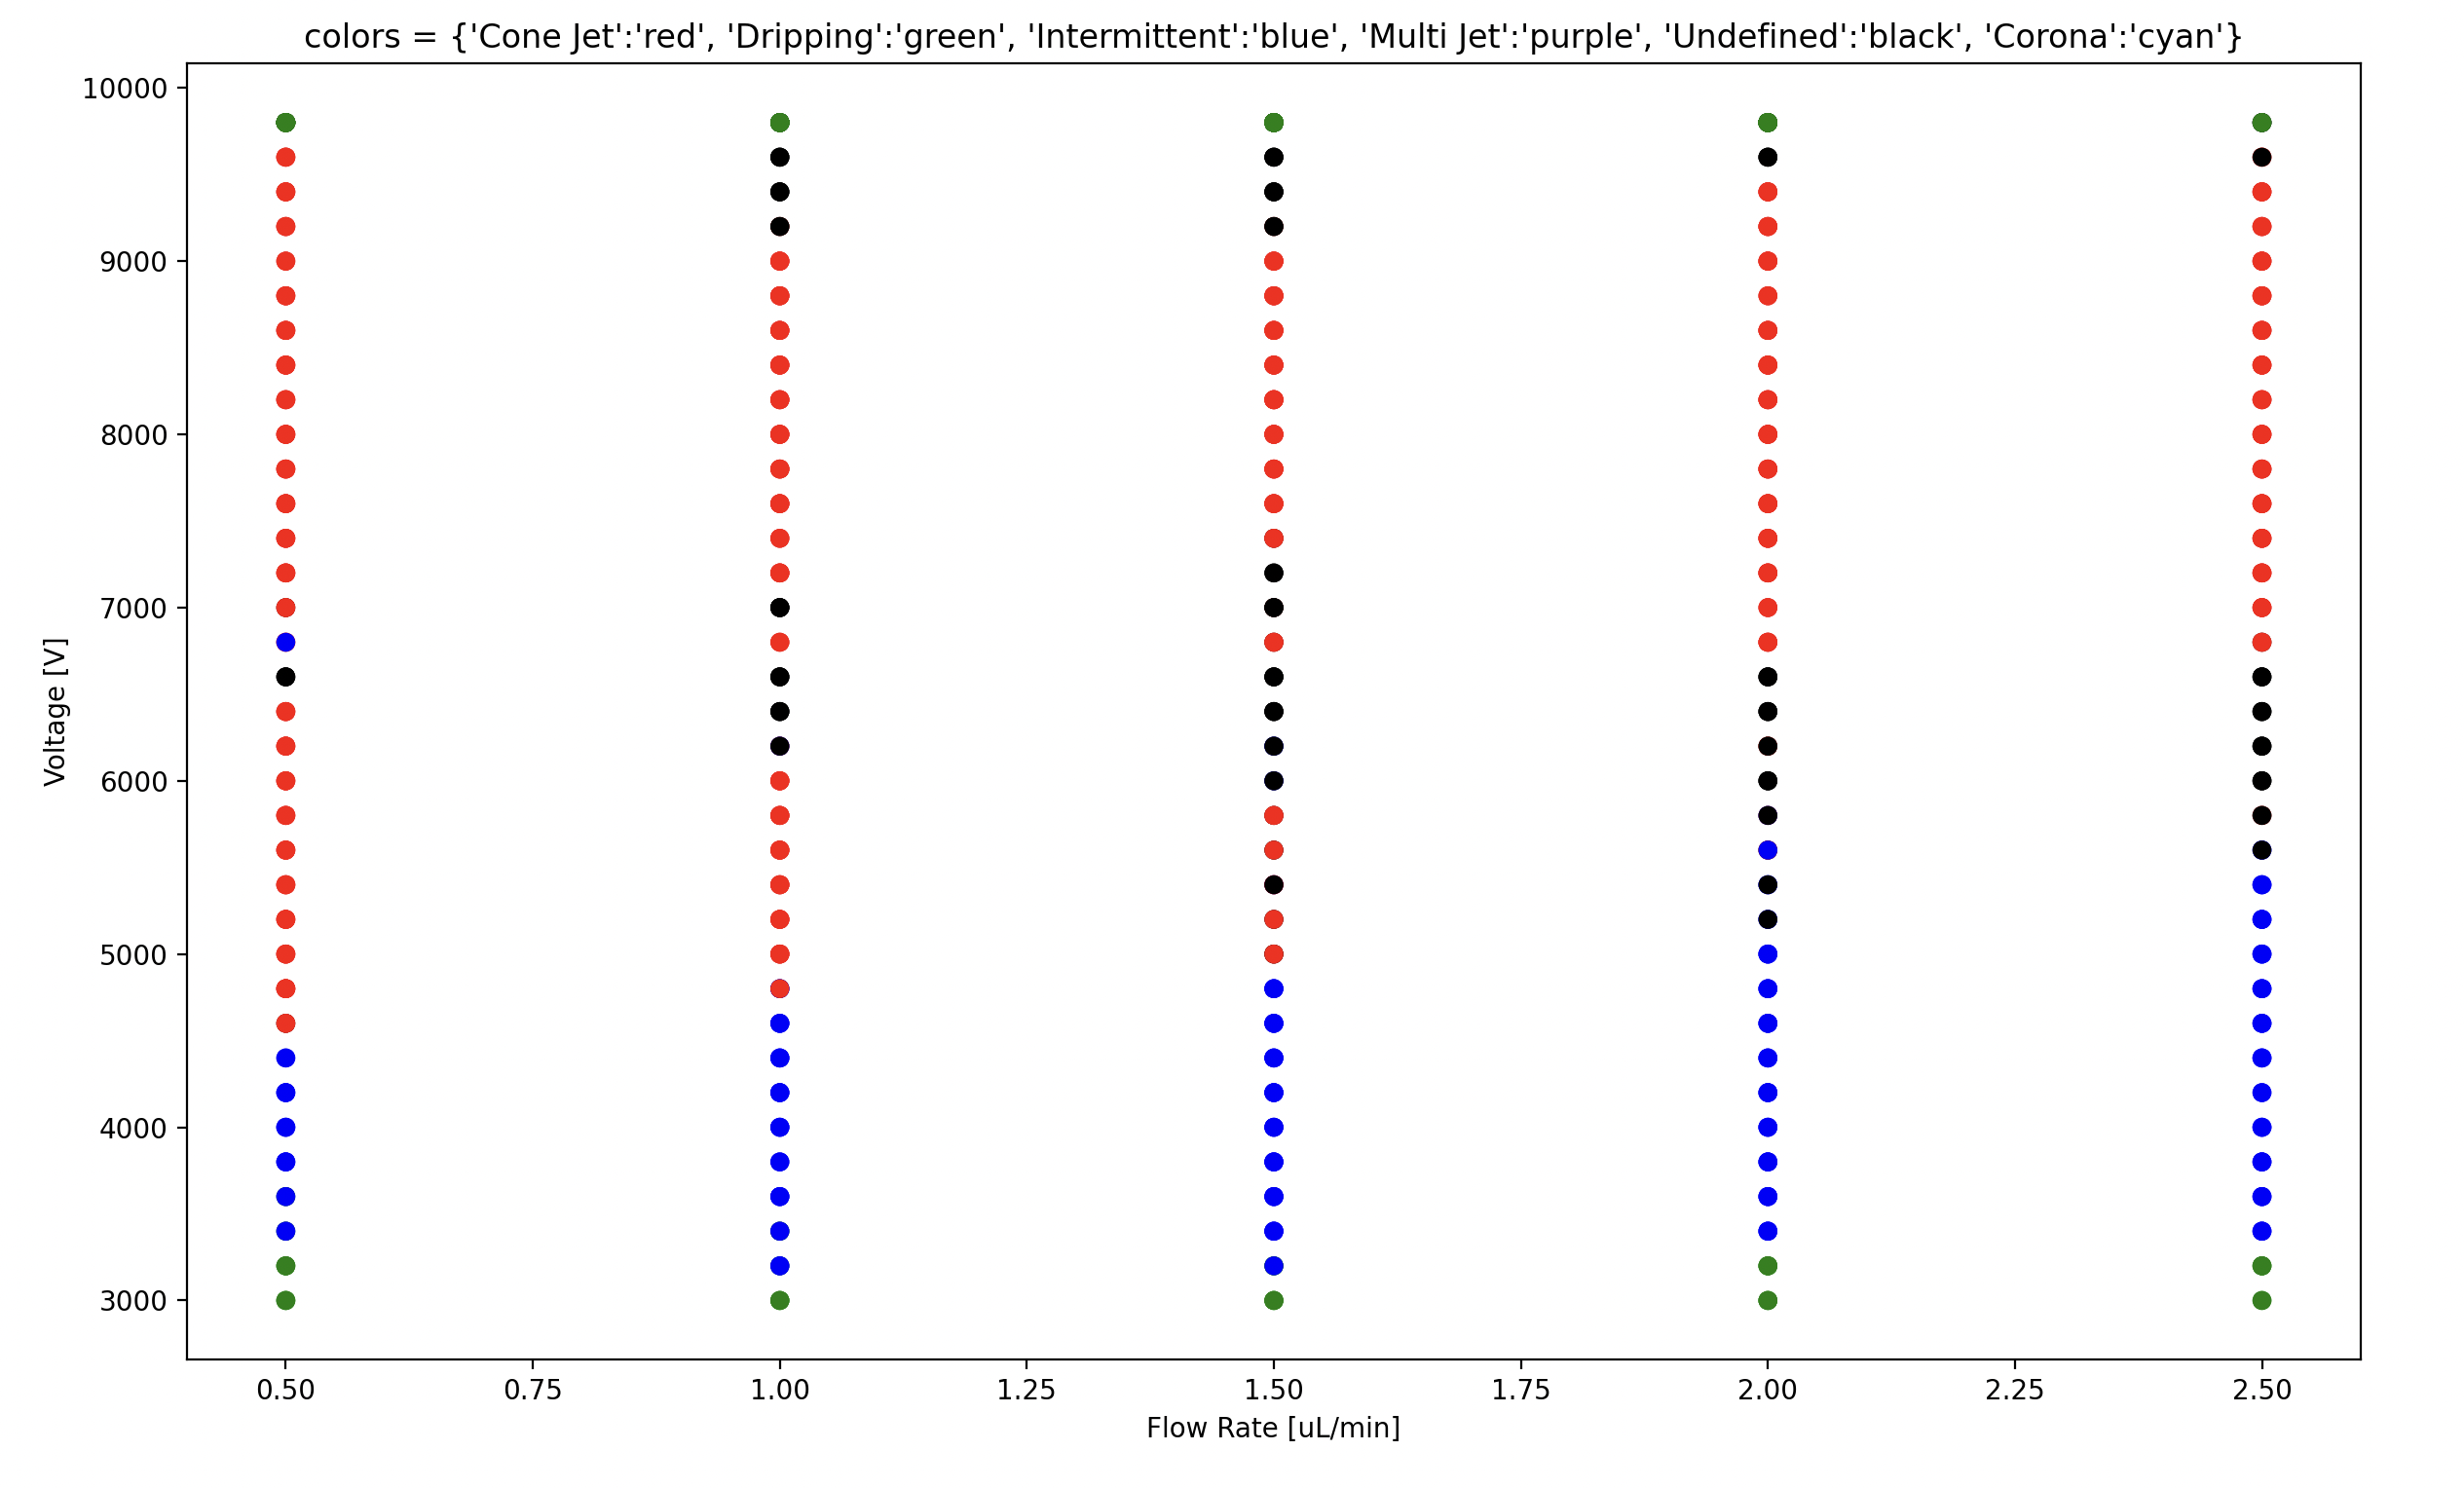
\includegraphics[width=15cm]{images/map1.png}
        \caption{First mapping trial}
    \end{figure}

    \begin{figure}[H]
        \center
        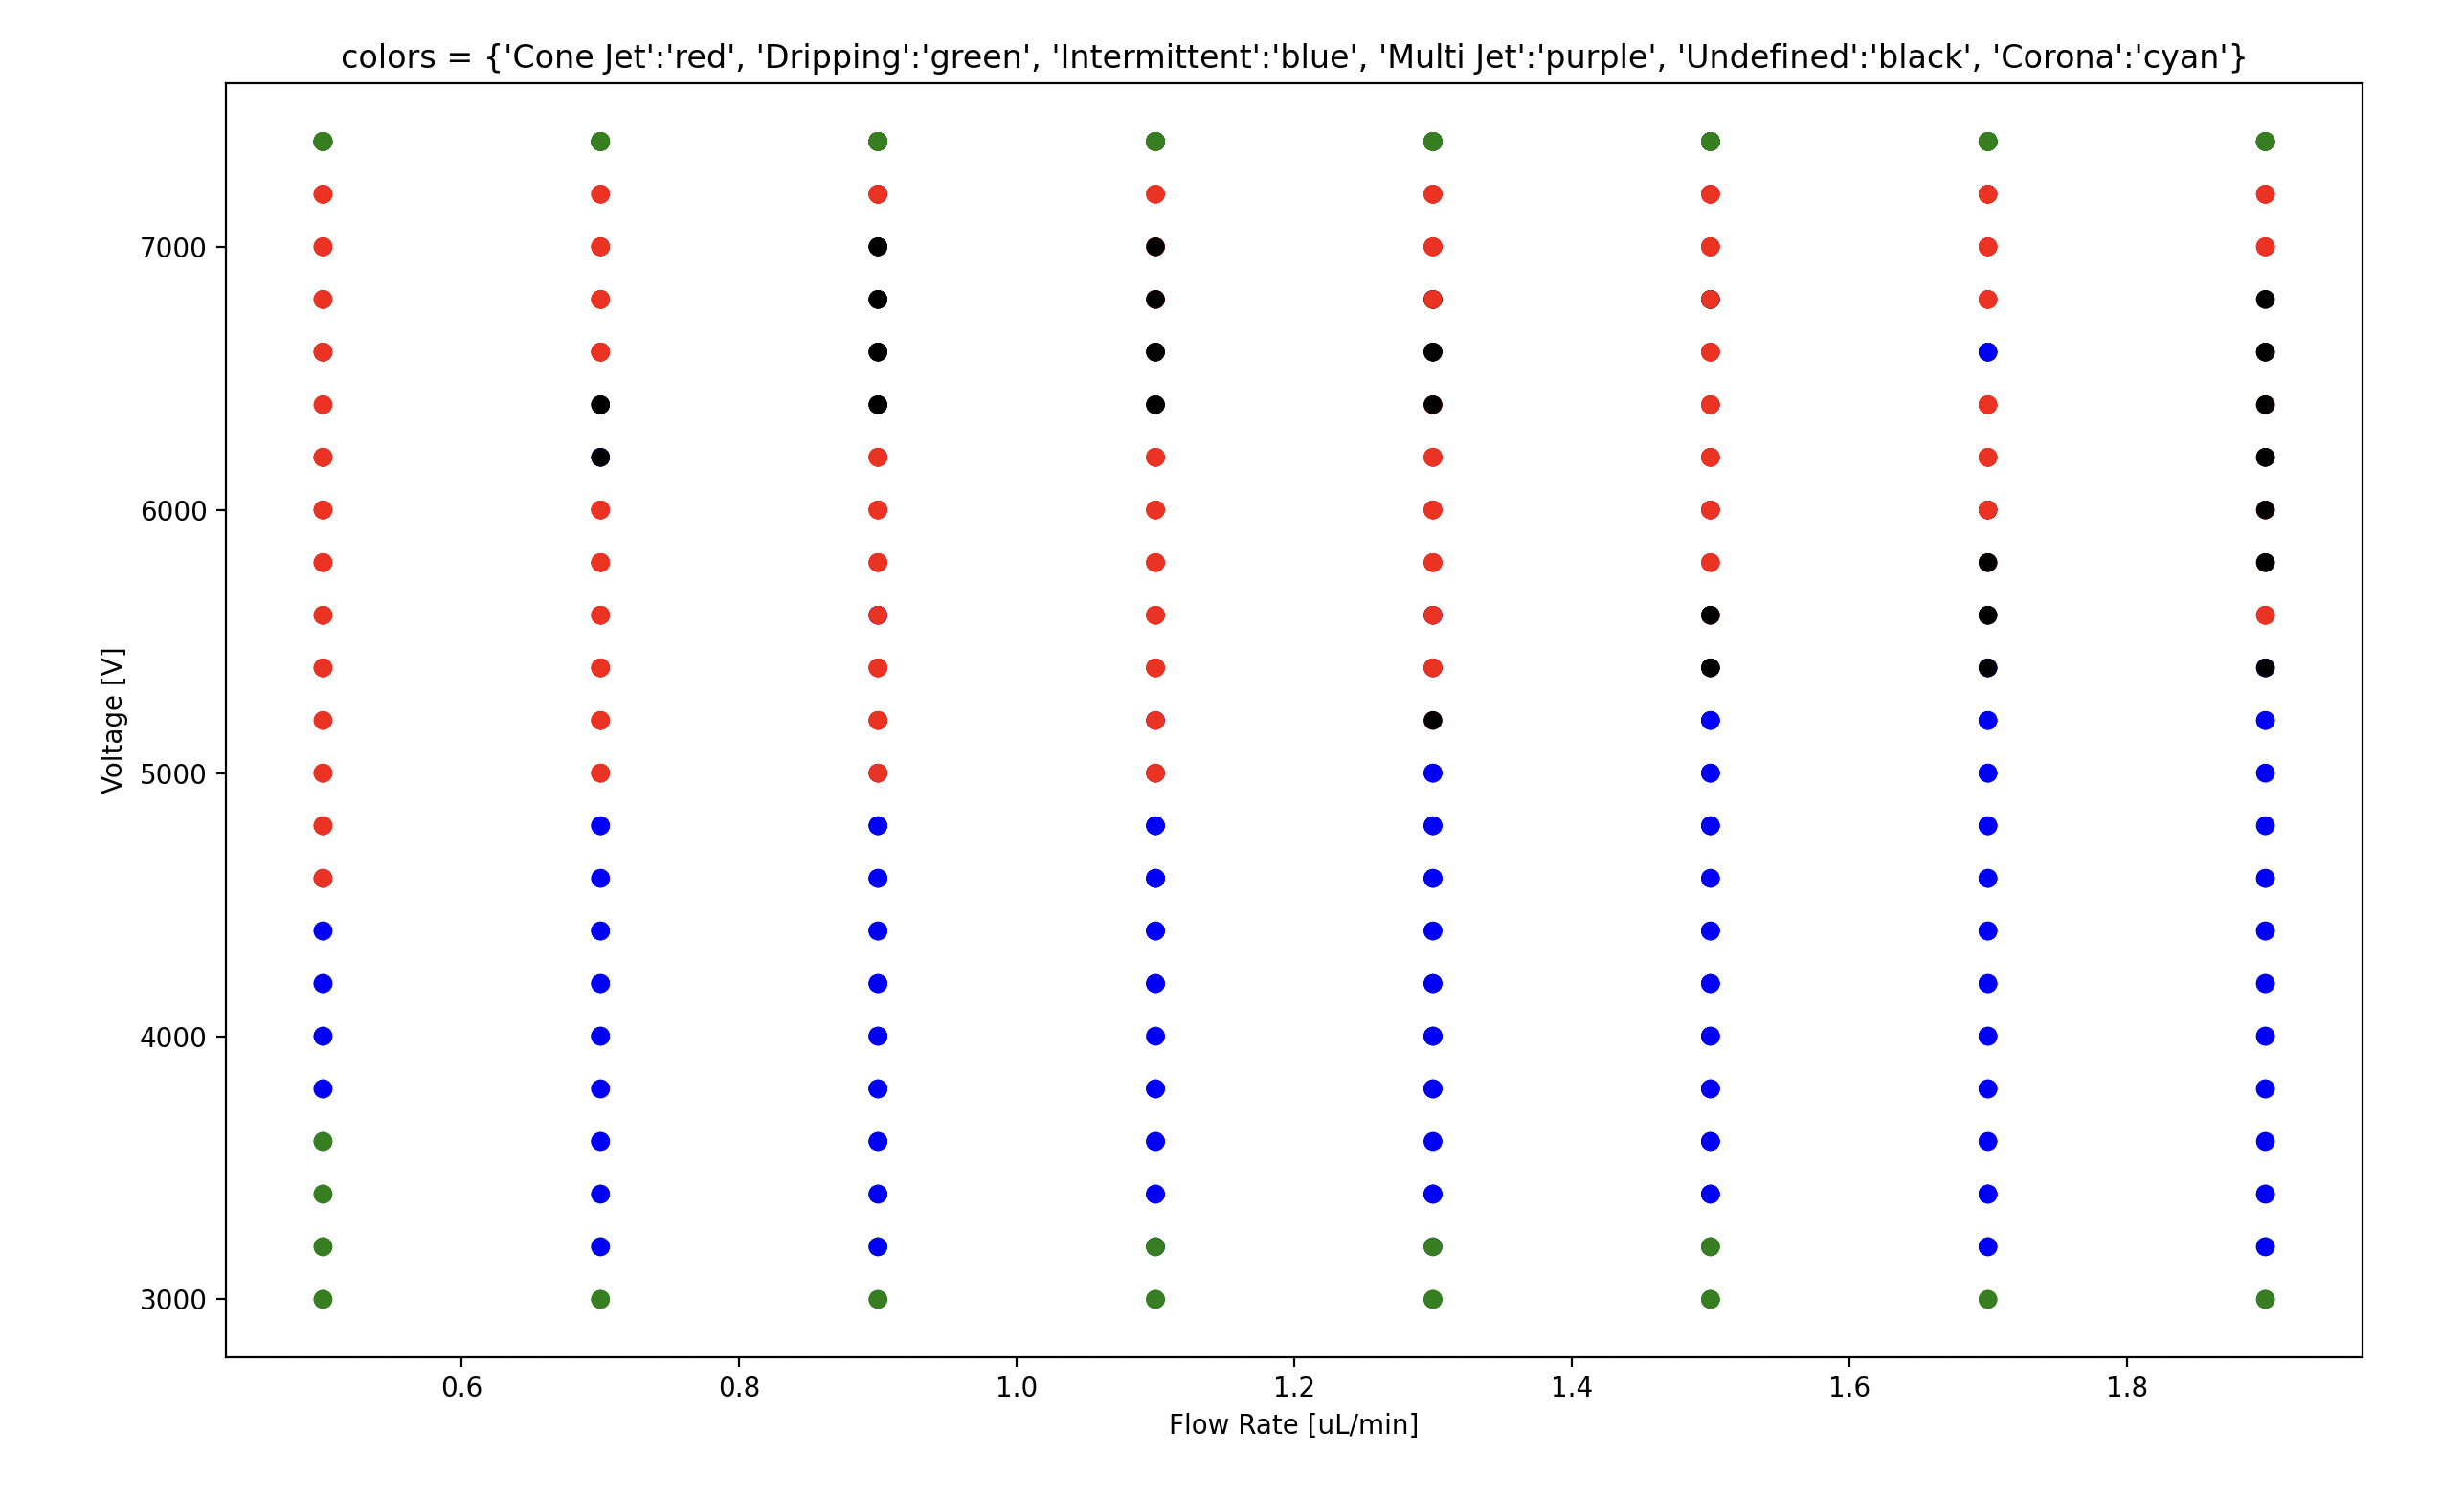
\includegraphics[width=15cm]{images/map2.png}
        \caption{Second mapping trial}
    \end{figure}

    It was noticed that the motor of the pump in certains speed generate a noise caused by the stepping from the stepper motor.
    This noise from the motor was being acquired by the current data and was interfering in the classification method.
    Because of that the firsts results of the map have a lot of undefined or incorrect classifications.
    This can be reduced inserting a bubble in the syringe to atenuate mechanical noises. 


    \begin{figure}[H]
        \center
        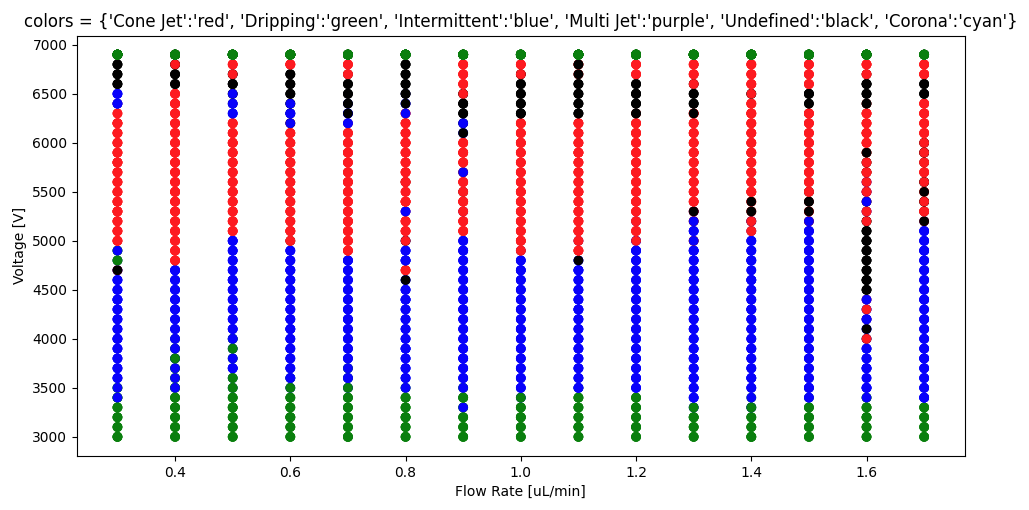
\includegraphics[width=15cm]{images/map3.png}
        \caption{map3}
    \end{figure}






\subsection*{3.3 Capacitance of the system in step response}

    We were discussing if the voltage step implies in a transient state in the current acquired.
    If yes, the data acquired in this transient should not be used in the classification step. Since we want to analise
    the spraying in a constant dynamics.

    \begin{multicols}{2}

        \begin{figure}[H]
            \center
            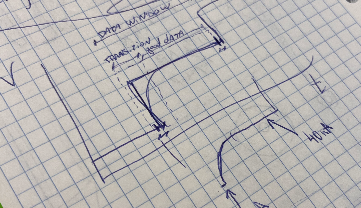
\includegraphics[width=8cm]{images/idea.png}
            \caption{ map3 reproccessed data head }
        \end{figure}


        For that I reproccessed all raw data acquired cutting the head of the data window. The new classification map is showed in the figure 10.

        \begin{figure}[H]
            \center
            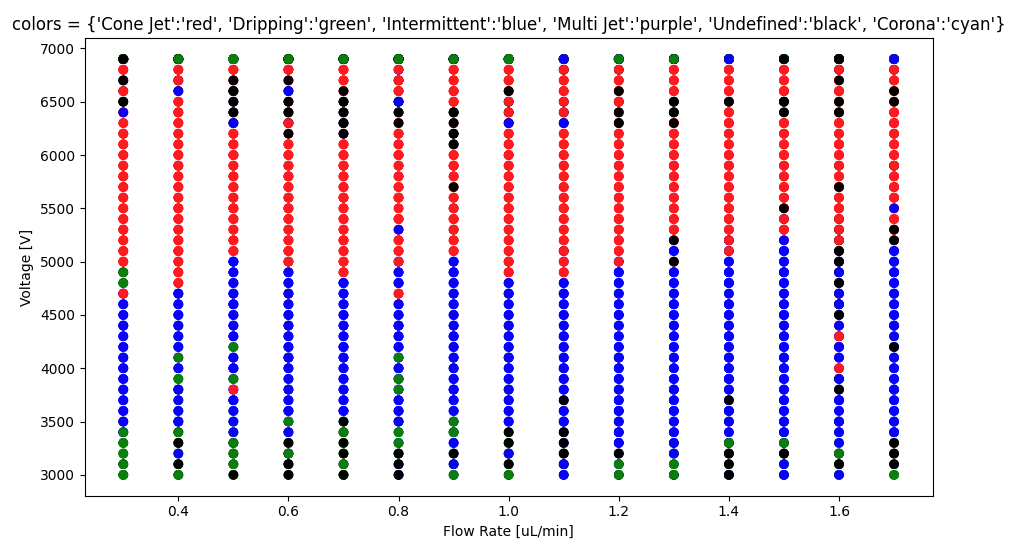
\includegraphics[width=8cm]{images/map3_reproccessed_data_head.png}
            \caption{ map3 reproccessed data head }
        \end{figure}

        Also tested cutting the tail of the data window to see if have improvements in the classification.

        \begin{figure}[H]
            \center
            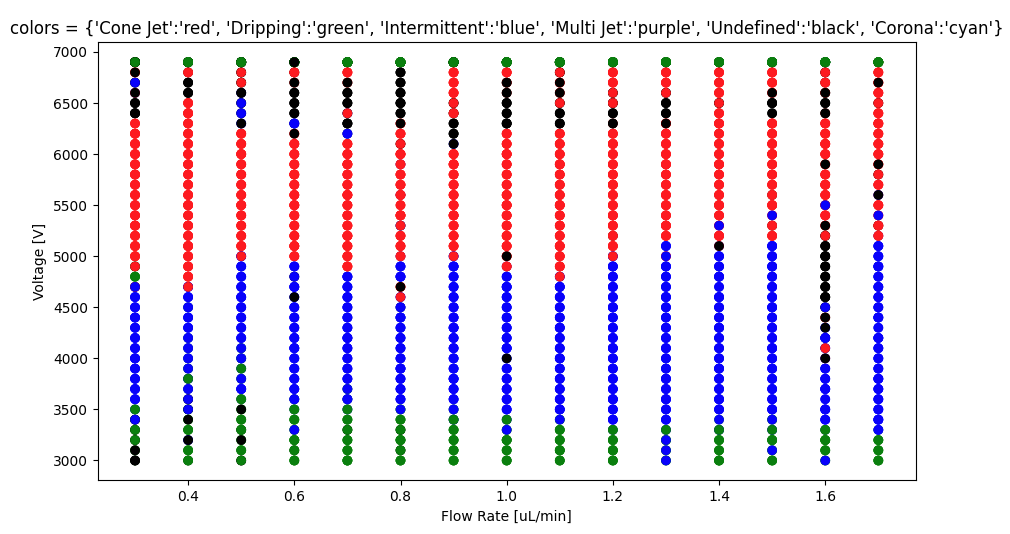
\includegraphics[width=8cm]{images/map3_reproccessed_data_tail.png}
            \caption{ map reproccessed data tail }
        \end{figure}


        \begin{figure}[H]
            \center
            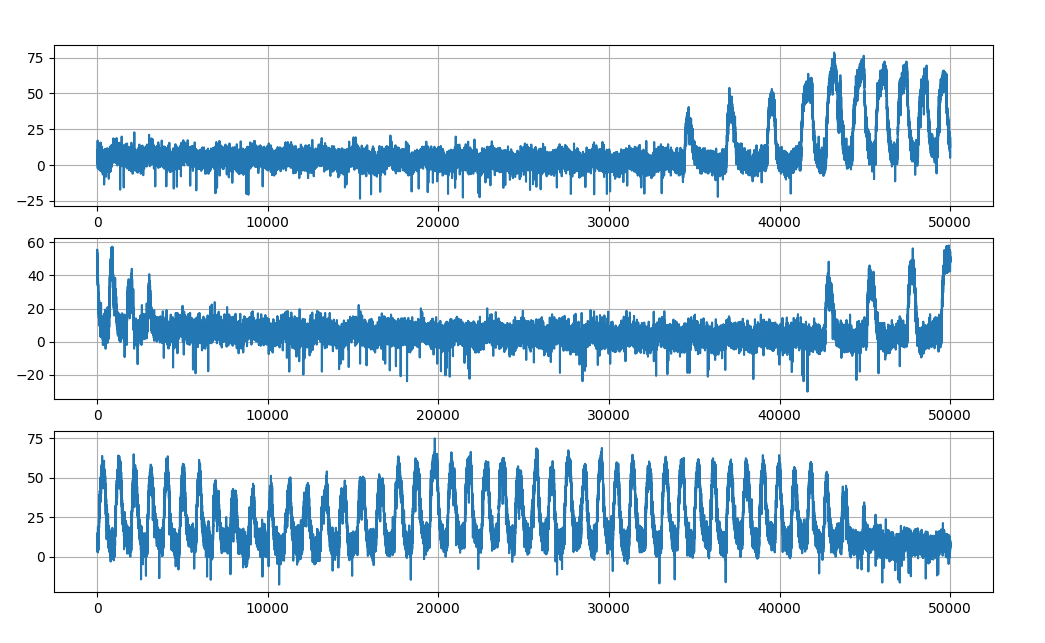
\includegraphics[width=8cm]{images/data_samples.png}
            \caption{ USE ANOTHER IMAGE WITH STABLE SAMPLES OR DELETE THIS ONE }
        \end{figure}

    \end{multicols}

    {TRY TO PUT STEP RESPONSE OF THE POWER SUPPLY HERE}


    CONCLUSION: Does not made much difference. For steps under 250V the system does not show a transition dynamic. 
    With steps above 250V the capacitance of the system reacts with a capacitance curve.



\subsection*{3.4 Manual x Automatic Cone Jet stability island maps}

    Metodology

    \begin{figure}[H]
        \center
        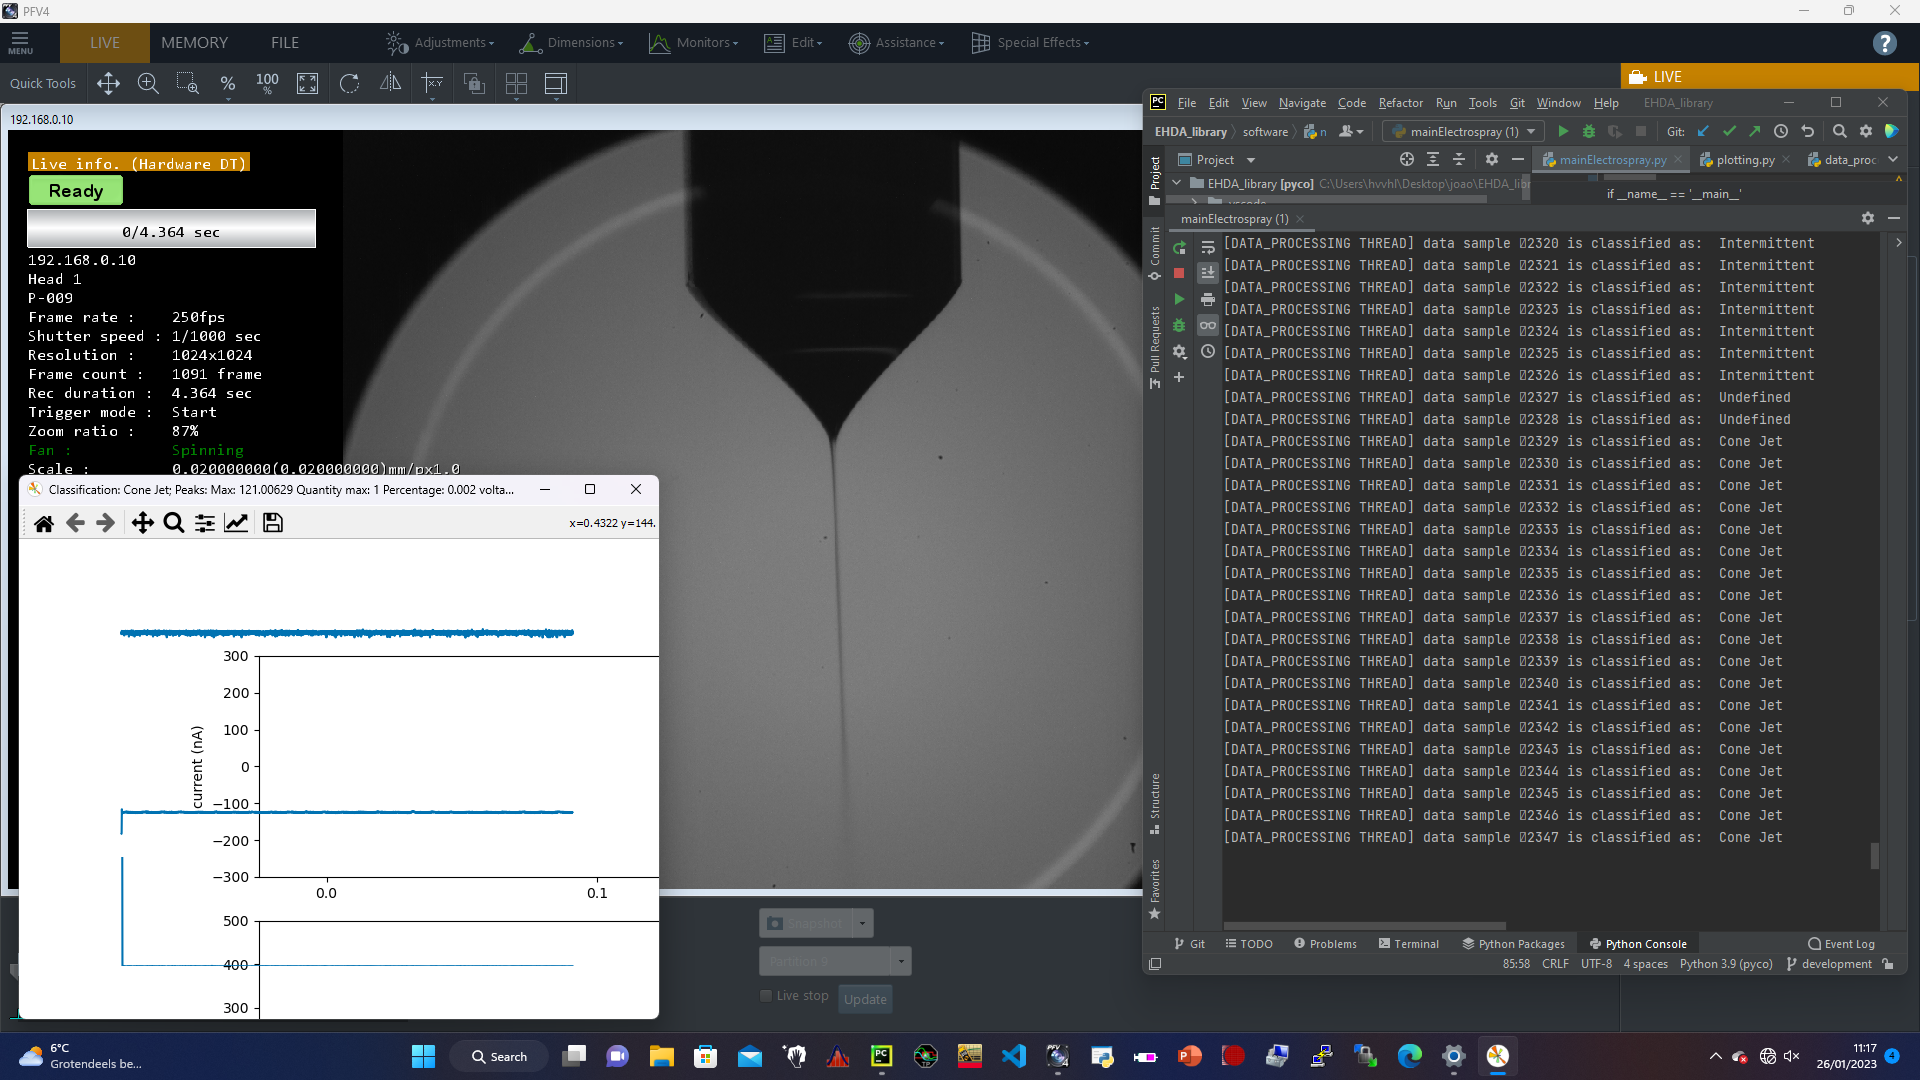
\includegraphics[width=14cm]{joao_26-01-22/screenshots/stableConeExp.png}
        \caption{exp 24}
    \end{figure}

    \begin{figure}[H]
        \center
        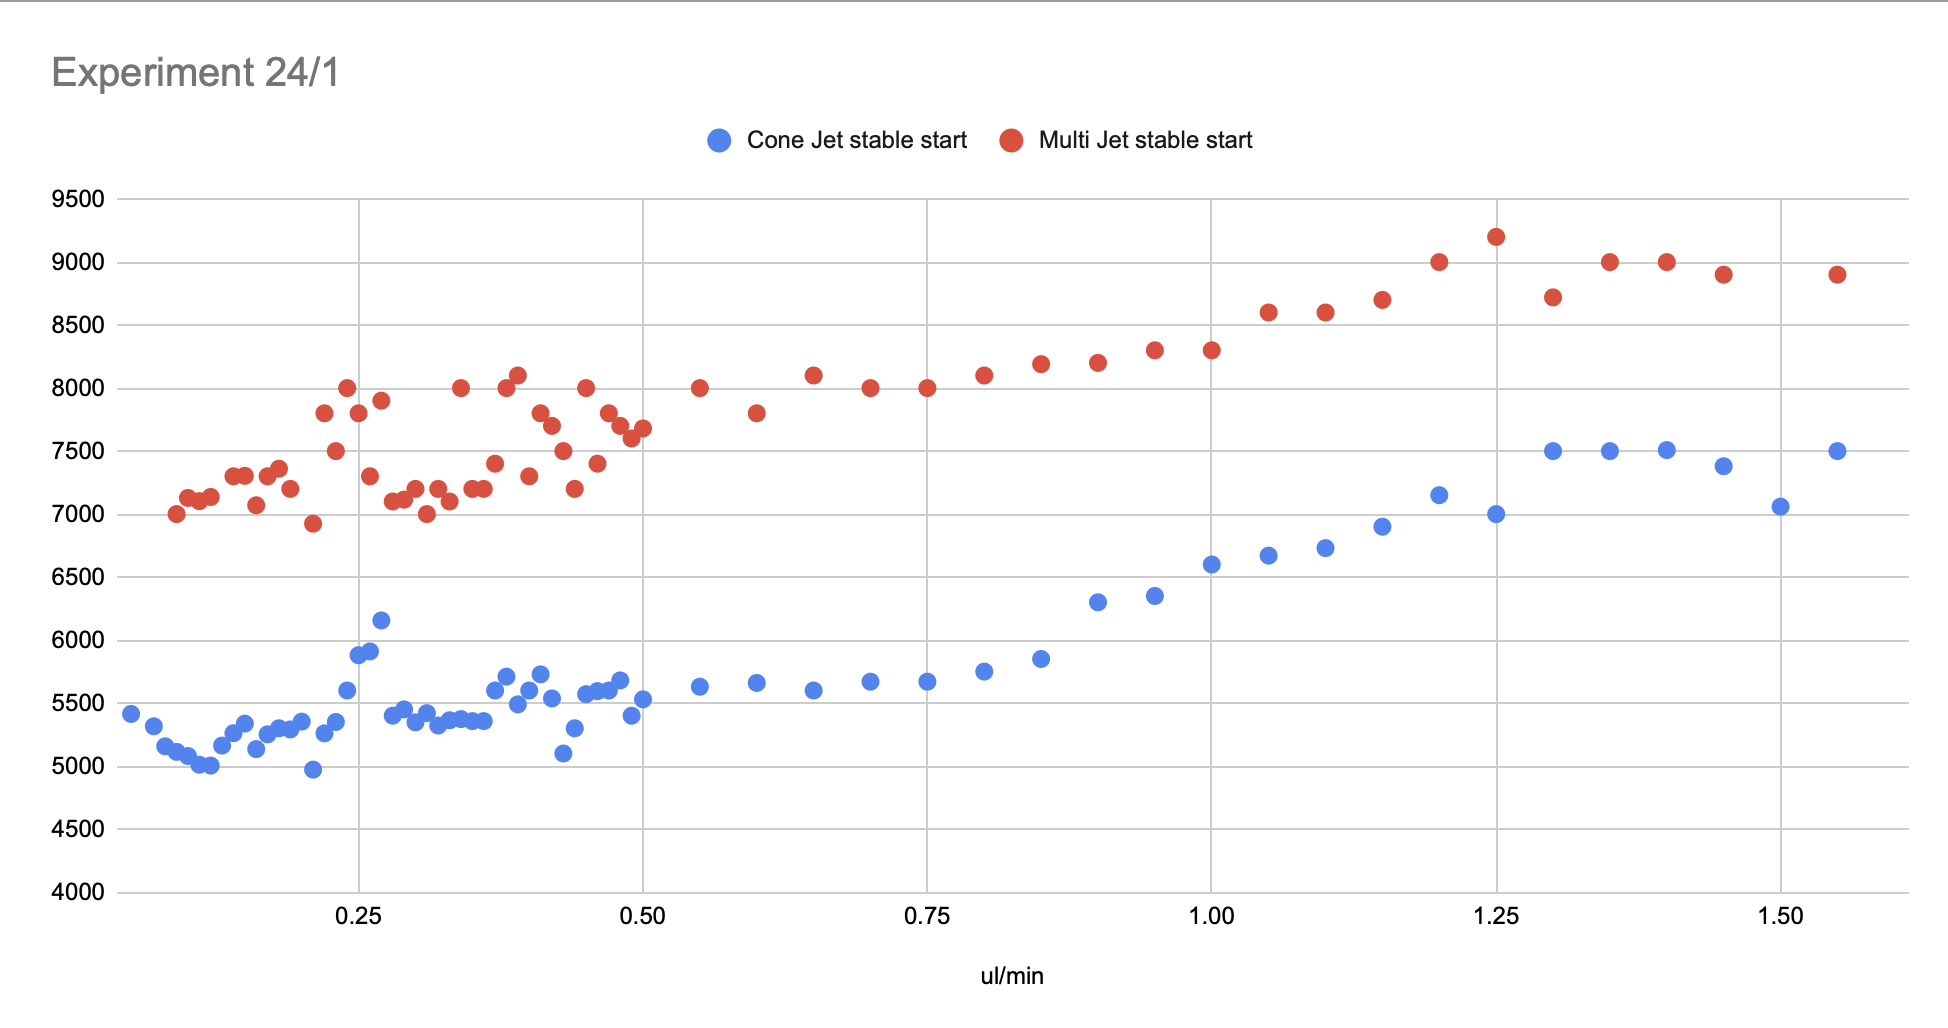
\includegraphics[width=8cm]{joao_26-01-22/epx_24-01.png}
        \caption{exp 24}
    \end{figure}

    \begin{figure}[H]
        \center
        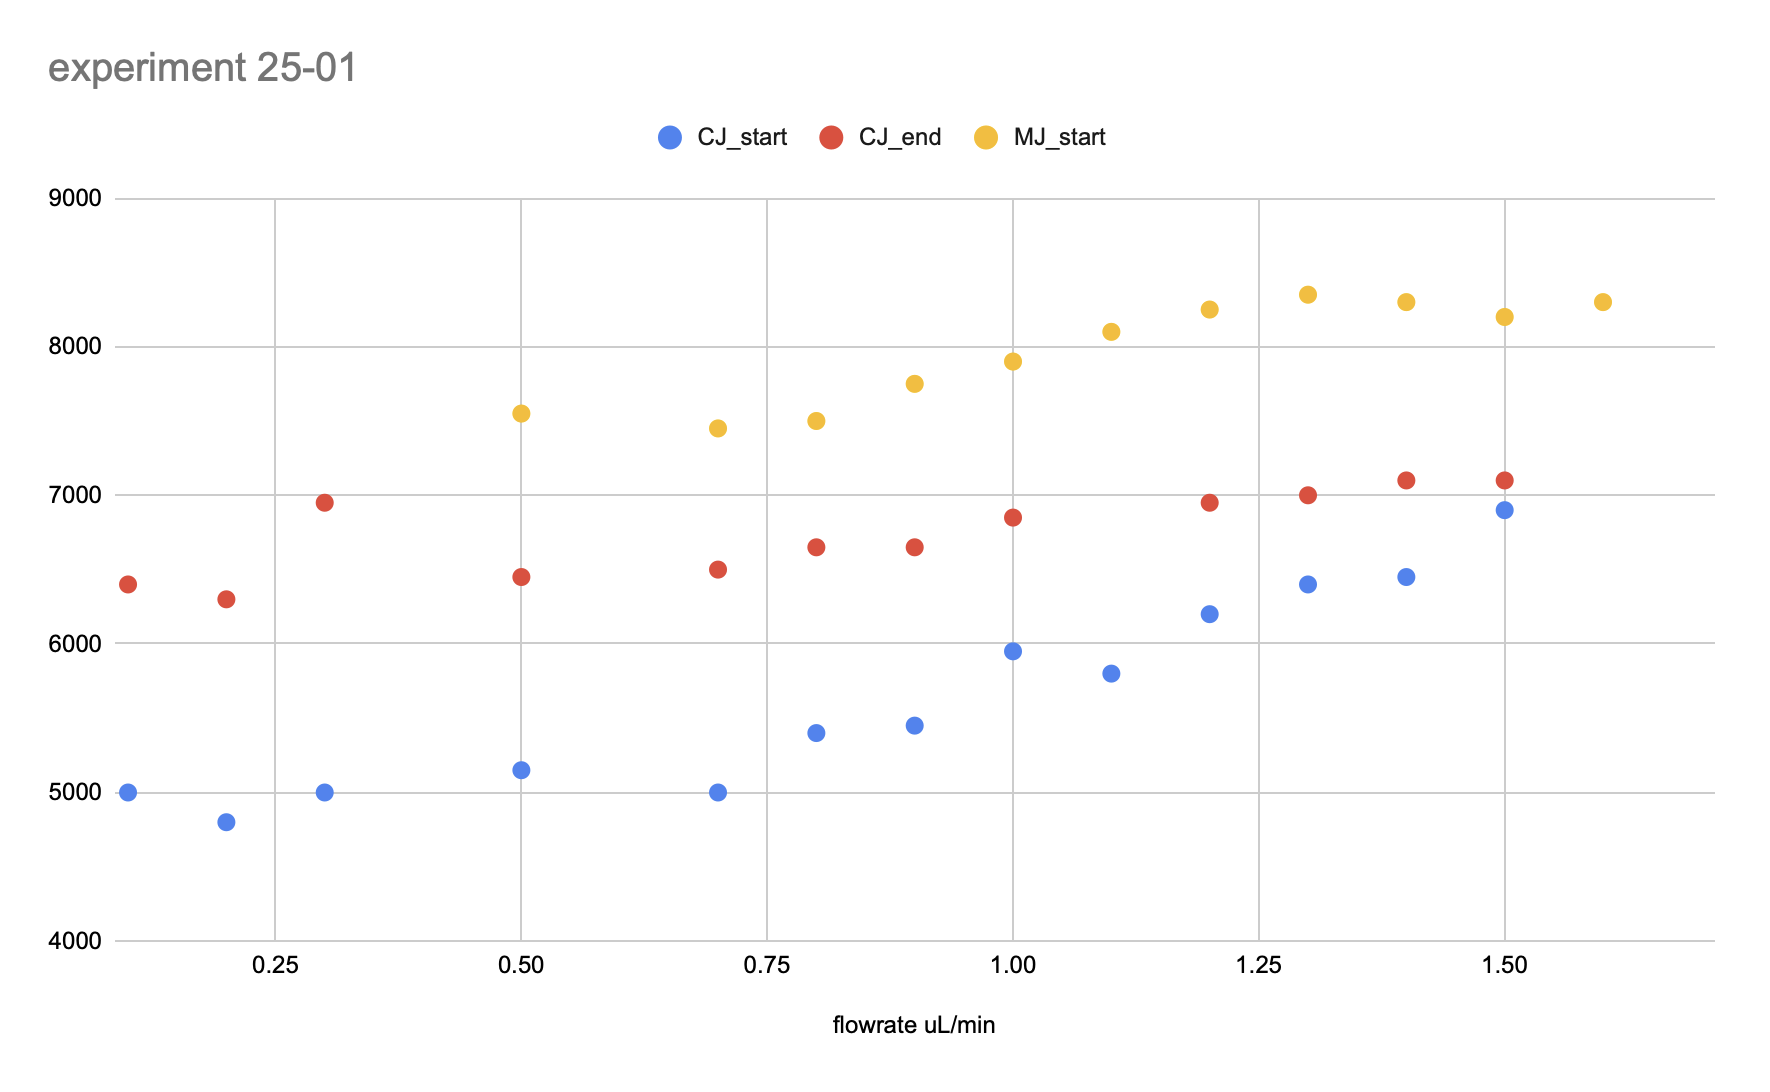
\includegraphics[width=8cm]{joao_26-01-22/exp25-01-1.png}
        \caption{ exp25-01-1 }
    \end{figure}

    \begin{figure}[H]
        \center
        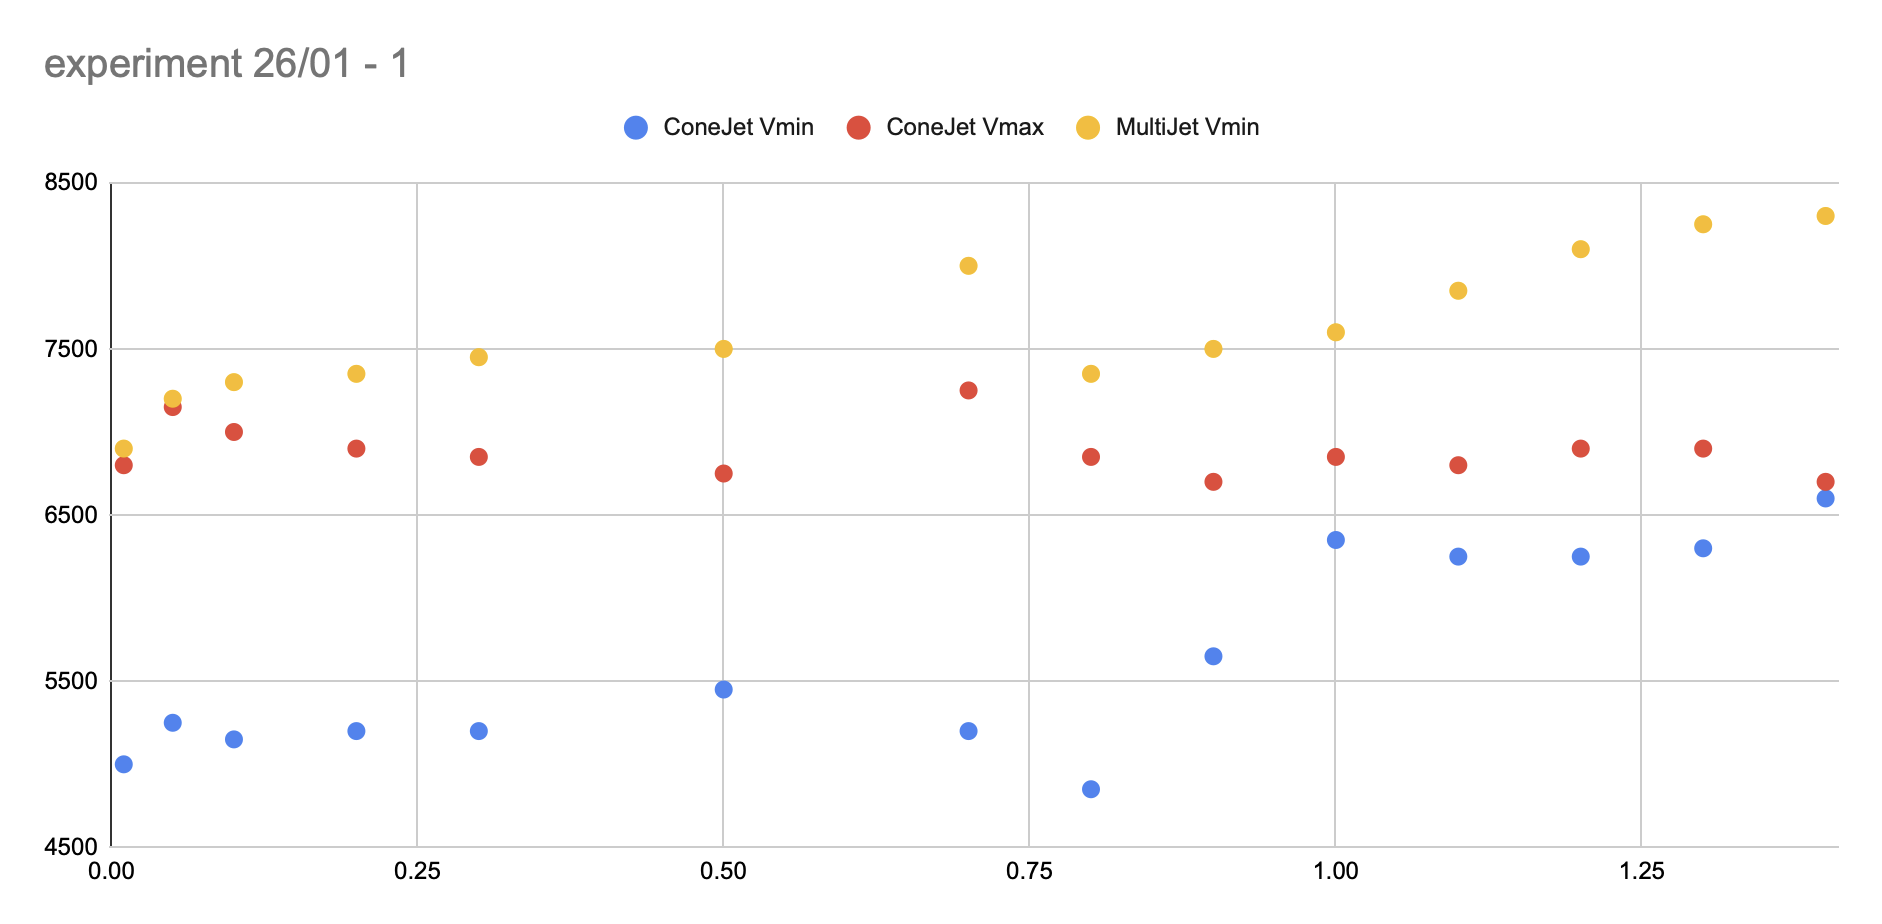
\includegraphics[width=8cm]{joao_26-01-22/exp-26-01-1.png}
        \caption{ exp-26-01-1 }
    \end{figure}

    \begin{figure}[H]
        \center
        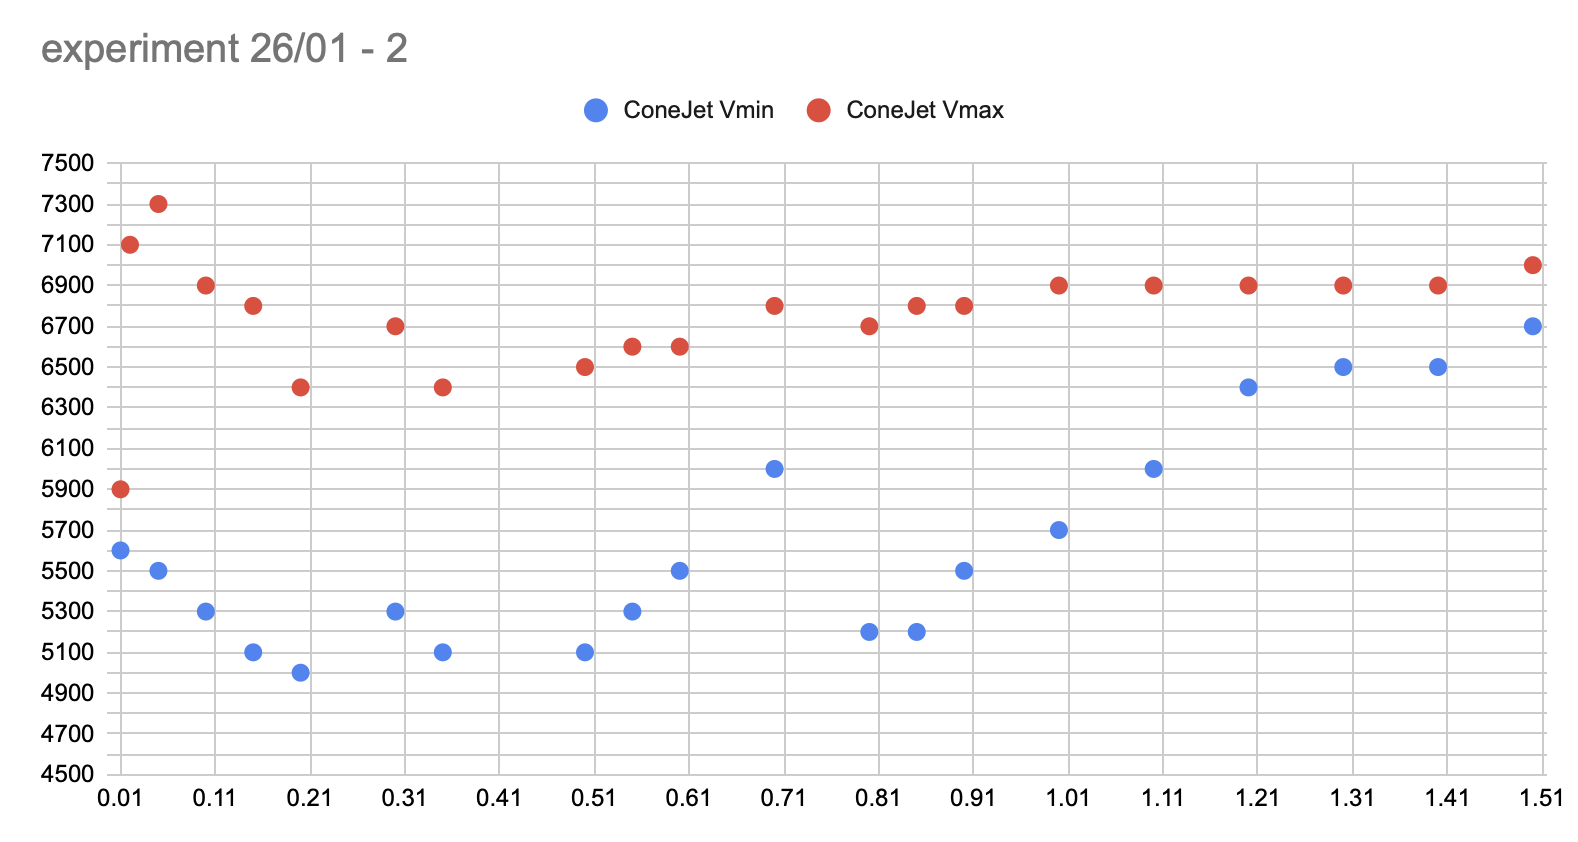
\includegraphics[width=8cm]{joao_26-01-22/exp26-01-2.png}
        \caption{ exp-26-01-2 }
    \end{figure}





\subsection*{3.5 Temperature and Humidity influences}

    - Started collecting temperature and humidity values for each sample using arduino and DHT11 sensor from adafruit.
    - Closed the system and sprayed pure oxygen O2 to decrease the humidity of the system.

